\chapter{Measurement of Directional Characteristics I}\label{ax:directional_1}
This appendix serves as a protocol to a series of measurements conducted on the 23\textsuperscript{rd} of February 2018 in the large anechoic chamber (B4-111) at the acoustical lab of Aalborg University at Fredrik Bajers Vej 7.\\
The goal of these measurements was to try out and evaluate a MATLAB-based measurement routine to quantify the directional characteristic of loudspeakers, especially gaining experience with determining the acoustical center of a loudspeaker.

\section*{Measuring Equipment and Materials}
The following measuring equipment was used:
\begin{itemize}[noitemsep]
\item Microphone \gls{bandk} 4144
\begin{itemize}[noitemsep]
\item AAU-number: 06552
\item Serial number: 297090
\end{itemize}
\item Preamplifier GRAS 26AK
\begin{itemize}[noitemsep]
\item AAU-number: 56525
\item Serial number: 32811
\end{itemize}
\item Power supply \gls{bandk} 2804
\begin{itemize}
\item AAU-number: 06998
\item Serial number: 455309
\end{itemize}
\item Calibrator \gls{bandk} 4231
\begin{itemize}[noitemsep]
\item AAU-number: 33691
\item Serial number: 2115338
\end{itemize}
\item Power Amplifier Pioneer A-616
\begin{itemize}[noitemsep]
\item AAU-number: 08249
\item Serial number: HJ9404841S
\end{itemize}
\item Sound card RME Fireface UCX
\begin{itemize}[noitemsep]
\item AAU-number: 108230
\item Serial number: 23811948
\end{itemize}
\item Turntable: Outline ET 250-3D
\begin{itemize}
\item Serial number: REIBO012
\end{itemize}
\item MATLAB r2017b on OSX 10.11.6
\item Loudspeaker SEAS 33 F-WKA
\end{itemize}

The following material was used:
\begin{itemize}[noitemsep]
%\item \SI{1/2}{\inch} to \SI{1}{\inch} preamp adapter
\item Microphone clip
\item Microphone stand
\item LEMU cable
\item XLR cable
\item Ethernet cable
\item Loudspeaker stand
\item Loudspeaker cabinet, plywood, outside dimensions: (400x400x400)\SI{}{\milli\meter}, wall thickness: \SI{20}{\milli\meter}
\end{itemize}

\section*{Setup}
A sketch of the measurement setup can be found in \autoref{fig:measurement_setup}. A picture is given in \autoref{fig:setup_02_23}

\begin{figure}[htbp]
	\centering
	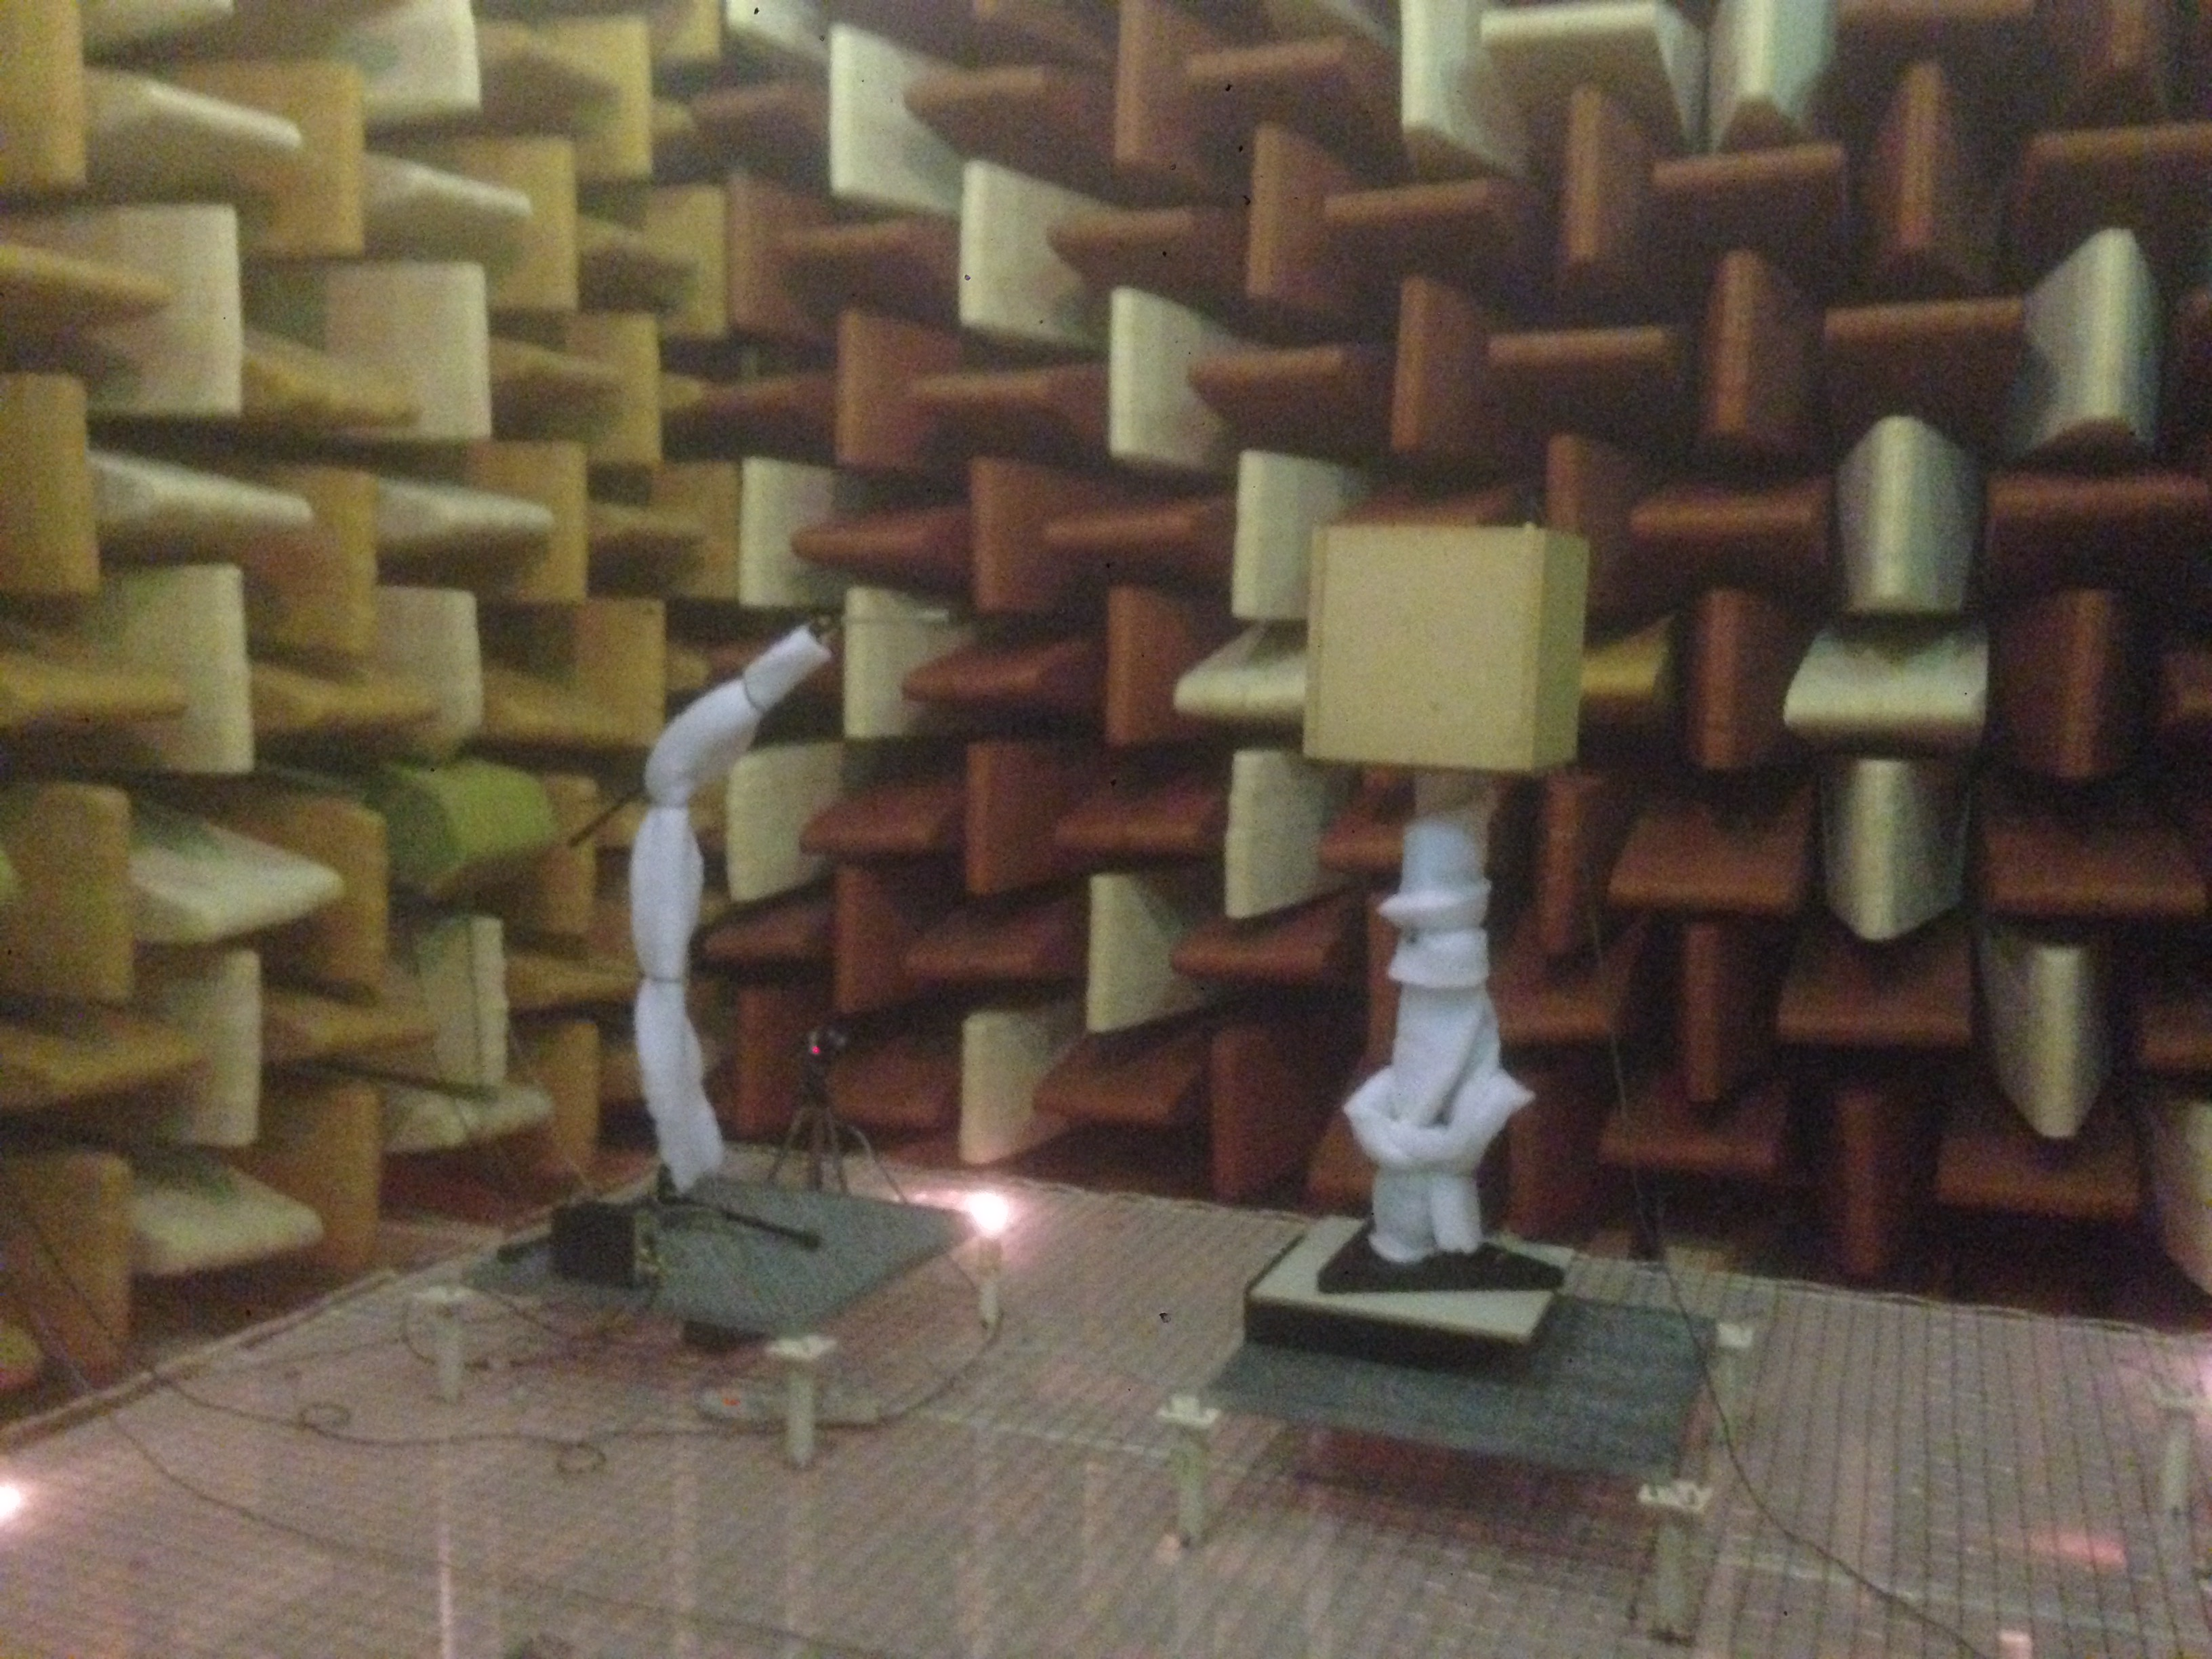
\includegraphics[width=0.7\textwidth]{02_23_setup.JPG}
	\caption{Measurement setup}
		\label{fig:setup_02_23}
\end{figure}

The horizontal distance between the microphone and the edge of the cabinet was \SI{0.75}{\meter}. This rather short distance was deliberately chosen for the sake of testing the measurement setup and getting an idea of the position of the acoustic center of the speaker. Directivity measurements should be conducted in the far field. In the frequency range that this project is covering, this means, that loudspeaker and microphone have to be placed significantly further apart. Because of the early stage of development, in which the measurement routine was at the point in time, that the measurement took place, no output calibration was applied. This means, that all measurement results are only relative and have no link to physical units that have been measured.

\section*{Results}
The measurement results have to be viewed remembering, that this measurement series has to be considered a practice run before the actual measurement to characterize the directivity characteristics of the speaker. \autoref{fig:02_23_pressure} shows the results of a measurement conducted at a distance \(d=\) \SI{0.75}{\meter} to the front plane of the speaker. The \gls{spl} normed to the level on the main axis is displayed along the radial coordinate. The angular coordinate describes the position of the microphone in relation to the main axis of the speaker. The coloured lines relate to different frequencies.
The shape of the \SI{60}{\hertz} curve appears to be quite similar to a circle. However, it is not concentric with the pole. Several reasons seem likely to cause this behaviour.  First of all the distance between the microphone and the speaker does not correspond to far field conditions in this frequency range. Secondly, the speaker may not behave as an ideal omnidirectional source and at last the acoustical center of the speaker might have been misplaced off the rotational axis of the turn table.\\
It can be seen, that the pressure on the back side of the speaker keeps decreasing for rising frequencies, especially around approx. \SI{120}{\degree} and \SI{240}{\degree}.

\begin{figure}[htbp]
	\centering
	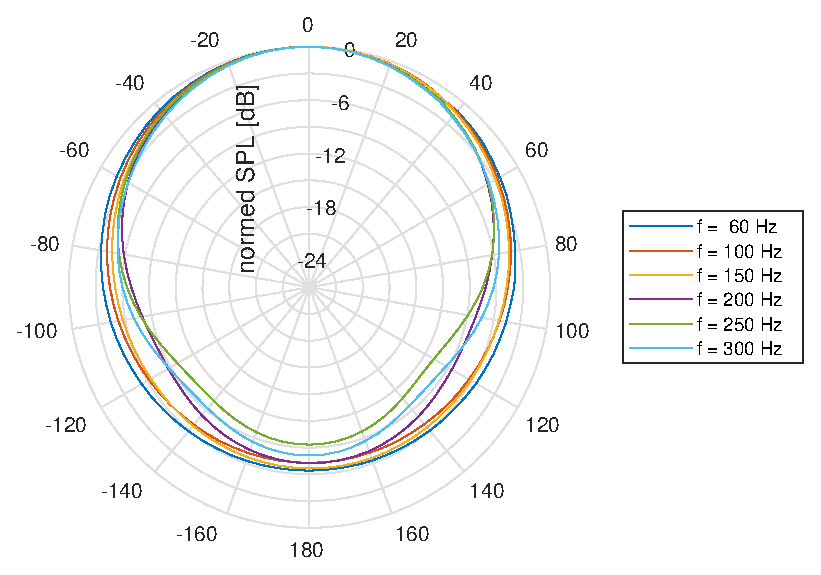
\includegraphics[width=0.7\textwidth]{02_23_pressure.eps}
	\caption{Normed \gls{spl}, measured at a distance \(d=\)\SI{0.75}{\meter}}
		\label{fig:02_23_pressure}
\end{figure}

In order to further investigate the position of the acoustical center in relation to the rotational axis of the turntable, a look at \autoref{fig:02_23_phase} might yield more information. The phase displayed along the radial coordinate. The colours correspond to the same frequencies as in \autoref{fig:02_23_pressure}. It has to be noted, that the phase angle, that is shown in the plot does not necessarily represent the phase angle of the sound pressure related to the motion of the loud speaker membrane, because the phase characteristic of the auto interface and the amplifier were not taken into account via calibration. The phase angles can therefore only be viewed relative to eachother. Similar to the \autoref{fig:02_23_pressure}, the graphs appear to be circular at least at the lower frequencies, but not concentric with the pole.\\
When interpreting these curves, one must take the definition of the acoustical center from \autoref{sec:ac_center} into account. Because the acoustical center is defined the position of a point source, it is to be expected that around a circumference around this point source the signal at any measurement point should be in phase. This would correspond to a concentric circle on the plot. The shifted circles in the polar plot indicate, that the acoustical center has been in front of the rotational axis of the turntable during the measurement. It might be possible to calculate the offset out of the phase data (see \autoref{sec:ac_center}). This however has to be verified in later measurements (see \autoref{ax:directional_2}).\\
The shape of the phase graph tends to look more like a cardiod towards higher frequencies. This might possibly be a general tendency but could also be influenced by the comparatively short distance between the microphone and the speaker. 

\begin{figure}[htbp]
	\centering
	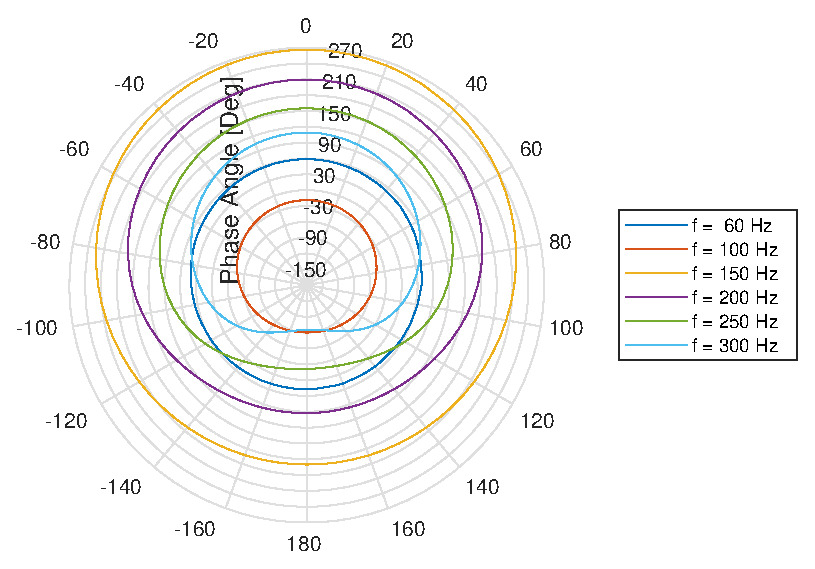
\includegraphics[width=0.7\textwidth]{02_23_phase.eps}
	\caption{Phase (uncalibrated), measured at a distance \(d=\)\SI{0.75}{\meter}}
		\label{fig:02_23_phase}
\end{figure}
